\documentclass[conference,onecolumn]{IEEEtran}

% Language setting
\usepackage[spanish]{babel}

\usepackage{ragged2e}

\IEEEoverridecommandlockouts
% The preceding line is only needed to identify funding in the first footnote. If that is unneeded, please comment it out.
\usepackage{cite}
\usepackage{amsmath,amssymb,amsfonts}
\usepackage{algorithmic}
\usepackage{graphicx}
\usepackage{textcomp}
\usepackage{xcolor}
\usepackage{blindtext}
\usepackage{float}
\usepackage{tabularx}
\usepackage{titlesec}
\usepackage{needspace}

\setlength{\abovedisplayskip}{4pt}
\setlength{\belowdisplayskip}{4pt}

\def\BibTeX{{\rm B\kern-.05em{\sc i\kern-.025em b}\kern-.08em
    T\kern-.1667em\lower.7ex\hbox{E}\kern-.125emX}}
\begin{document}

\title{Implementación de Controlador Digital de Bajo Nivel para motores DC\\
{\footnotesize Laboratorio 1}}

\author{\IEEEauthorblockN{Leonardo Achá Boiano}
\IEEEauthorblockA{\textit{Ingenieria Mecatrónica: IMT 342} \\
\textit{Universidad Católica Boliviana}\\
Santa Cruz de la Sierra, Bolivia \\
leonardo.acha@ucb.edu.bo}
}

\maketitle
\justifying 

\begin{abstract}
Este informe presenta la implementación de un controlador digital de bajo nivel para motores DC en el contexto de un laboratorio de ingeniería mecatrónica. El trabajo aborda desde la medición de la señal de entrada hasta la implementación y evaluación del controlador digital. Se describe el proceso de medición de la señal de entrada, la supervisión de modulación por ancho de pulsos (PWM) y la implementación del control en lazo abierto del motor DC. En la segunda parte del laboratorio, se desarrolla un sistema de lazo abierto para la planta, se diseña y sintoniza un controlador PID en configuración paralela, y se transfieren los parámetros a la planta real. Los resultados experimentales muestran el rendimiento del sistema en lazo cerrado frente a diferentes tipos de entrada, como señales sinusoidales y escalones. Este trabajo proporciona una visión completa de la implementación de controladores digitales para motores DC en aplicaciones mecatrónicas.

\end{abstract}

\begin{IEEEkeywords}
Control, Motor, ESP32, PID, Matlab, Lazo Abierto, Lazo cerrado, Encoder.
\end{IEEEkeywords}

\section{Introducción}
En este informe se presenta la implementación de un controlador digital de bajo nivel para motores DC en el contexto de un laboratorio de ingeniería mecatrónica. Este trabajo se centró en comprender y aplicar conceptos clave de control, modulación por ancho de pulsos (PWM) y sistemas de lazo cerrado para optimizar el rendimiento y la precisión del motor DC. A lo largo del informe, se describen las etapas del proceso experimental, desde la medición de la señal de entrada hasta la implementación y evaluación del controlador digital, proporcionando una visión detallada de esta importante área de la ingeniería mecatrónica.

\section{Procedimiento}
La metodología empleada en el laboratorio se desarrolló de la siguiente manera. En primer lugar, se procedió a medir la señal de entrada por medio de la conexión wifi implementada en el microcontrolador, en este caso, el STM32. La señal de entrada era sinusoidal y provenía de un programa que simulaba un generador de señales analógico enviando la señal digitalizada con una resolución de 16 bits.

Posteriormente, se supervisó el funcionamiento correcto del módulo de modulación por ancho de pulsos (PWM) utilizando un osciloscopio para asegurar que el PWM generara la señal correctamente con una frecuencias variadas.

Luego, se implementó el control de pulsos del motor DC, lo que implicó calcular el ciclo de trabajo del PWM en función de la señal de entrada como se puede apreciar en la Figura~\ref{fig:encoder_signal}. Además, se determinó la dirección de rotación del motor en relación con el rango del ADC y se proporcionó el signo de la señal por separado.

El siguiente paso involucró el control de la velocidad y dirección de giro del motor, lo que se logró ajustando el ciclo de trabajo del PWM.

Para obtener el \textit{Bode Plot} de fase y amplitud de sistema de lazo abierto, se recopilaron los datos de la respuesta del sistema a una entrada de escalón, de la misma se extrajeron los parámetros del sistema.

En la segunda parte del laboratorio, centrado en la construcción del sistema de lazo cerrado, se sintetizó e implementó un controlador digital en la plataforma utilizando el modelo obtenido previamente en el sistema de lazo abierto para sintonizar el controlador en simulación. Este controlador se diseñó para cumplir con las especificaciones técnicas, incluido un \textit{overshoot} menor al 30\% y un error de sistema de e = 2° para una señal a 0.05 Hz.

Finalmente, se evaluó la calidad del sistema cerrado para asegurar que cumpliera con los requisitos técnicos establecidos.

\section{Resultados}

\subsection{Desarrollo de la Planta}

\begin{figure}[H]
    \centering
    \resizebox{0.6\textwidth}{!}{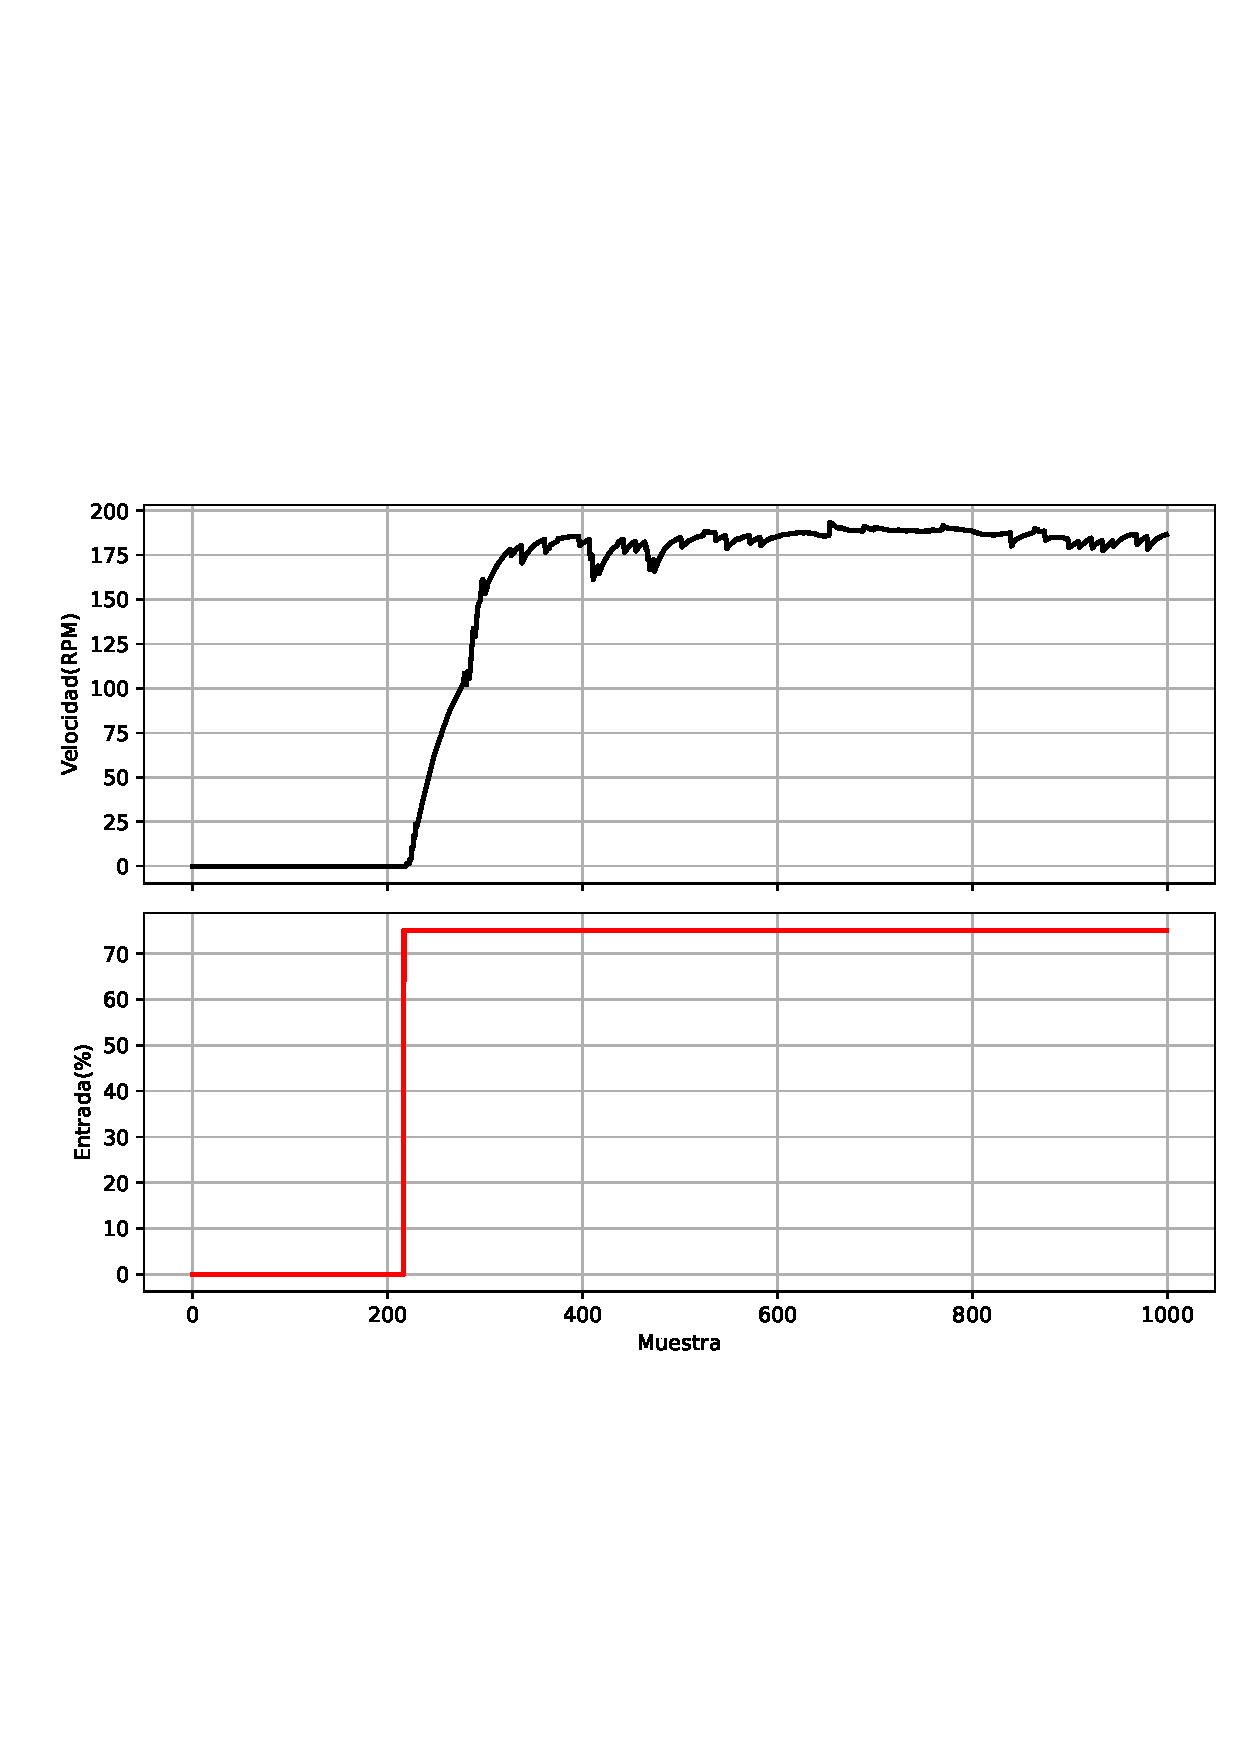
\includegraphics{images/Figure_1.jpg}}
    \caption{Señal del Encoder del Motor Visualizada en el Osciloscopio}
    \label{fig:encoder_signal}
\end{figure}

La Figura~\ref{fig:encoder_signal} presenta la señal del encoder del motor DC, capturada y visualizada en un osciloscopio. Esta representación gráfica es fundamental para entender cómo se traduce la posición del motor en una señal eléctrica. La forma de onda exhibida en el osciloscopio proporciona información sobre la velocidad y dirección del motor, lo que resulta crucial para el control y monitoreo del sistema. Se pudo calcular experimentalmente que el encoder del motor utilizado generaba un promedio de 480 pulsos por revolución. Se aproximó este numero a 512 para que sea potencia de 2 como suele ser el caso de los codificadores binarios.

\begin{figure}[H]
    \centering
    \resizebox{0.6\textwidth}{!}{\includegraphics{images/Figure_2_ewma_filter_04.png}}
    \caption{Respuesta del sistema en lazo abierto a una entrada escalón}
    \label{fig:open_loop_response}
\end{figure}

La Figura~\ref{fig:open_loop_response} muestra la respuesta del sistema en lazo abierto cuando se le aplica una señal de entrada en forma de escalón. Este gráfico es esencial para comprender el comportamiento intrínseco de la planta sin ningún controlador aplicado. Revela aspectos como el tiempo de respuesta, el sobre impulso y la estabilidad inherente del sistema. 
Notese que inicialmente la señal medida presentaba una cantidad significativa de ruido. A fin de mitigar este ruido se implementó un filtro digital de medias ponderadas.

\subsection{Identificación del Sistema}

\begin{figure}[H]
    \centering
    \resizebox{0.6\textwidth}{!}{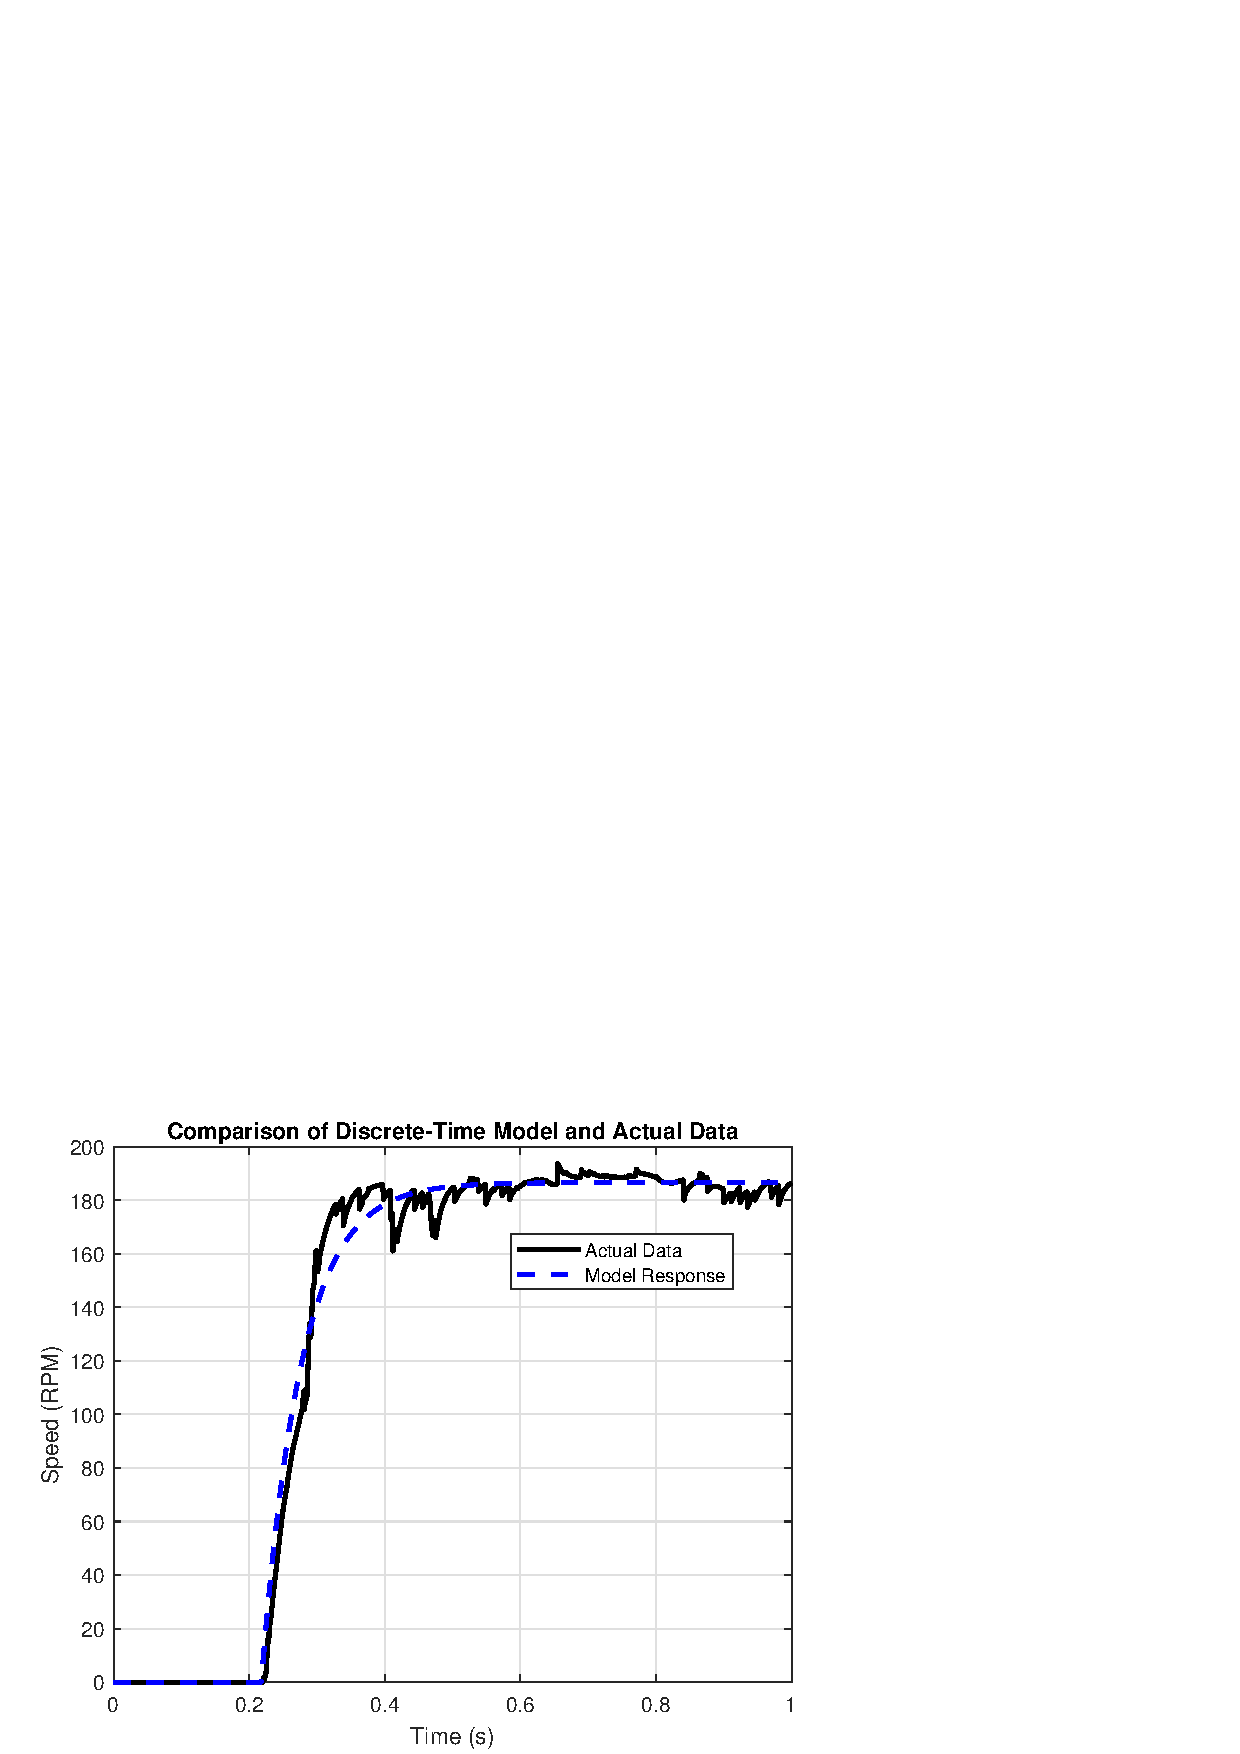
\includegraphics{images/Figure_3.png}}
    \caption{Identificación del Sistema}
    \label{fig:sistem_identification}
\end{figure}

En la Figura~\ref{fig:sistem_identification} se presenta el proceso de identificación del sistema. 
Mediante \textit{system identification} de matlab se idéntico los parámetros de la planta y se discreto la misma mediante el método de sostenedor de orden cero.
A través de este procedimiento, se obtienen los parámetros característicos de la planta, lo que incluye su respuesta en frecuencia y sus dinámicas.

\begin{equation}
\frac{0.04234 z^{-1}}{1 - 0.983 z^{-1}}
\end{equation}


\subsection{Implementación del Controlador}

Una vez identificado el sistema, procedimos a seleccionar un controlador. En este caso, optamos por el controlador PID en configuración paralela debido a su facilidad para ser sintonizado mediante métodos prácticos, sin requerir cálculos complejos. Como se observa en las ecuaciones siguientes, empleamos la aproximación de Tustin para discretizar este controlador. Luego, afinamos los parámetros del controlador mediante simulación. Finalmente, transferimos los parámetros a la planta, corrigiendo las discrepancias inherentes entre el modelo simulado y la planta real para minimizar los errores.

\begin{align}
C(s) &= K_p + \frac{K_i}{s} + K_d s \label{eq:1} \\
s &= 2T_s \cdot \frac{z - 1}{z + 1} \label{eq:2} \\
C(s) &= \frac{U(s)}{E(s)} = K_p + \frac{K_i}{\frac{2}{T_s} \cdot \frac{z - 1}{z + 1} + K_d \cdot \frac{2}{T_s} \cdot \frac{z - 1}{z + 1}} \label{eq:3} \\
C(s) &= \frac{2(z - 1)(z + 1)K_pT_s + KiT_s^2(z + 1)^2 + 4Kd(z - 1)^2}{2(z - 1)(z + 1)T_s} \label{eq:4} \\
a &= 2K_pT_s \label{eq:5} \\
b &= KiT_s^2 \label{eq:6} \\
c &= 4K_d \label{eq:7} \\
d &= 2T_s \label{eq:8} \\
\frac{U(z)}{E(z)} &= \frac{2(z - 1)(z + 1)K_pT_s + KiT_s^2(z + 1)^2 + 4Kd(z - 1)^2}{2(z - 1)(z + 1)T_s} \label{eq:9} \\
\frac{U(z)}{E(z)} &= \frac{a(z - 1)(z + 1) + b(z + 1)^2 + c(z - 1)}{2d(z - 1)(z + 1)} \label{eq:10} \\
\frac{U(z)}{E(z)} &= \frac{az^2 - a + bz^2 + 2bz + b + cz^2 - 2cz + c}{d(z^2 - 1)} \label{eq:11} \\
\frac{U(z)}{E(z)} &= \frac{(a + b + c)z^2 + 2(b - c)z + (b + c - a)}{d(z^2 - 1)} \label{eq:12} \\
\frac{U(z)}{E(z)} &= \frac{(a + b + c) + 2(b - c)z^{-1} + (b + c - a)z^{-2}}{d(1 - z^{-2})} \label{eq:13} \\
u(k) &= \frac{(a + b + c)}{d}e(k) + \frac{2(b - c)}{d}e(k - 1) + \frac{(b + c - a)}{d}e(k - 2) + u(k - 2) \label{eq:14}
\end{align}


\begin{figure}[H]
    \centering
    \resizebox{0.6\textwidth}{!}{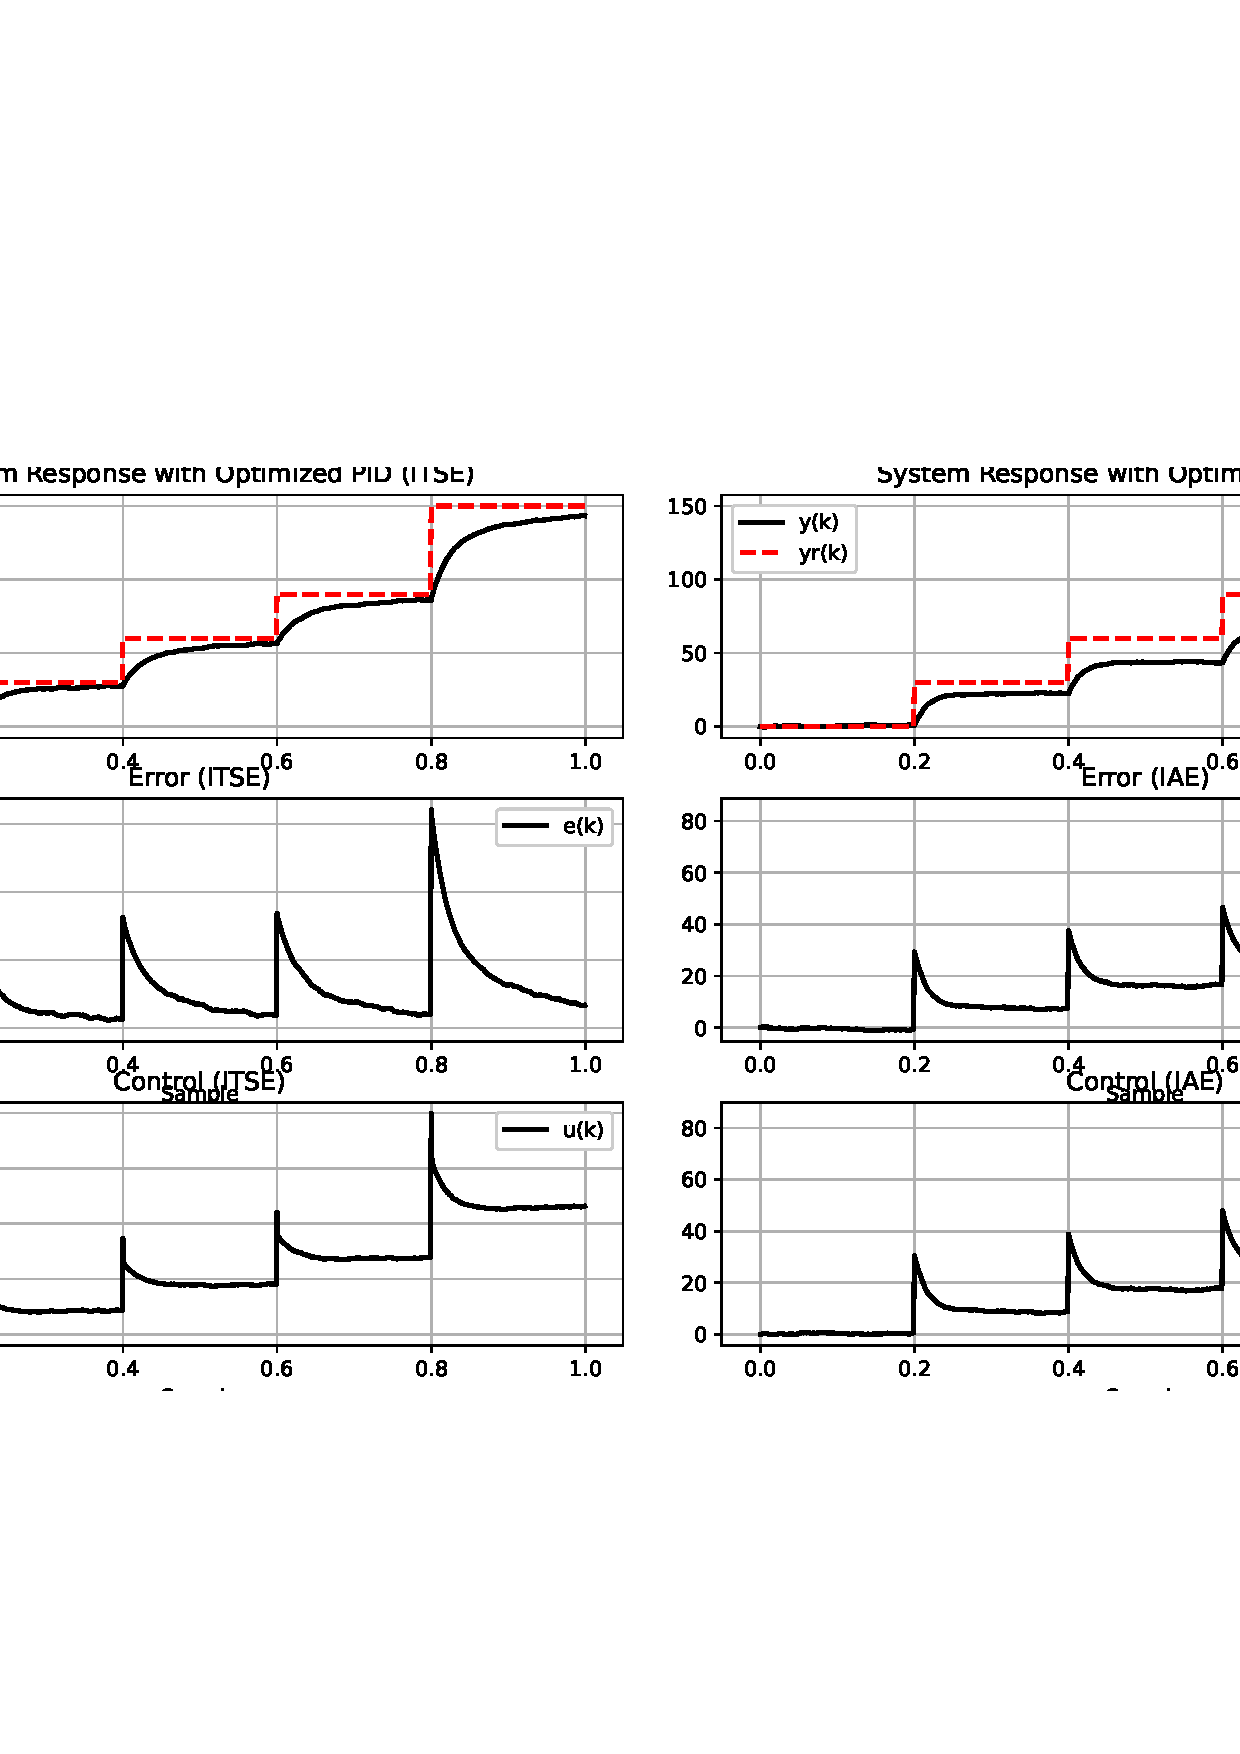
\includegraphics{images/Figure_4.png}}
    \caption{Simulación del Sistema en lazo cerrado a entrada Escalón}
    \label{fig:close_loop_response_simulation}
\end{figure}

La Figura~\ref{fig:close_loop_response_simulation} ilustra la simulación del sistema en lazo cerrado en respuesta a una entrada de tipo escalón. Esta simulación es crucial para evaluar y afinar el comportamiento del sistema controlado antes de implementarlo en la planta física. Proporciona una visión anticipada de cómo responderá el sistema real bajo control.

\begin{figure}[H]
    \centering
    \resizebox{0.6\textwidth}{!}{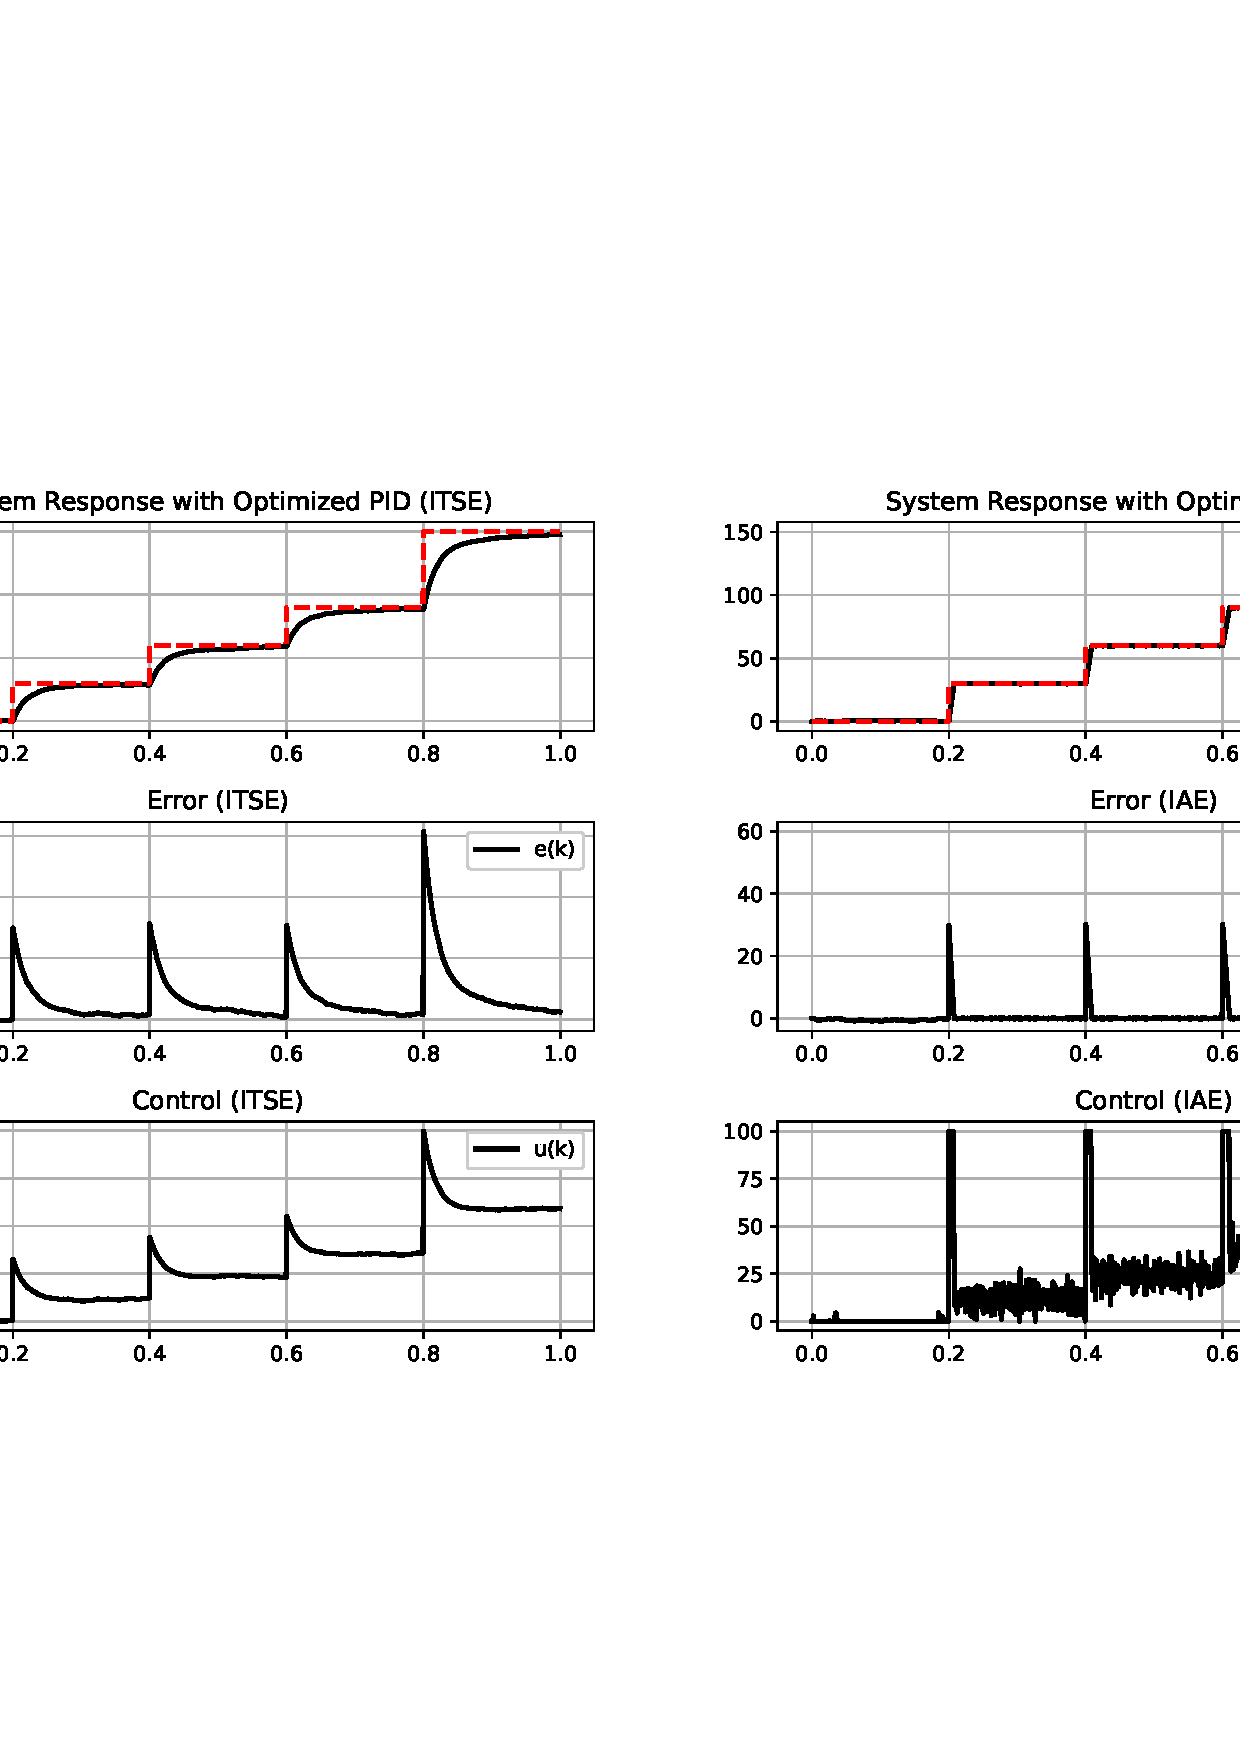
\includegraphics{images/Figure_5.png}}
    \caption{Calibración de los Parámetros del Controlador con la planta en funcionamiento}
    \label{fig:close_loop_pid_calibration}
\end{figure}
En la Figura~\ref{fig:close_loop_pid_calibration} se describe el proceso de calibración de los parámetros del controlador mientras la planta está en funcionamiento. Este paso crítico garantiza que el controlador se ajuste de manera óptima a las características y dinámicas específicas de la planta real.

\begin{figure}[H]
    \centering
    \resizebox{0.6\textwidth}{!}{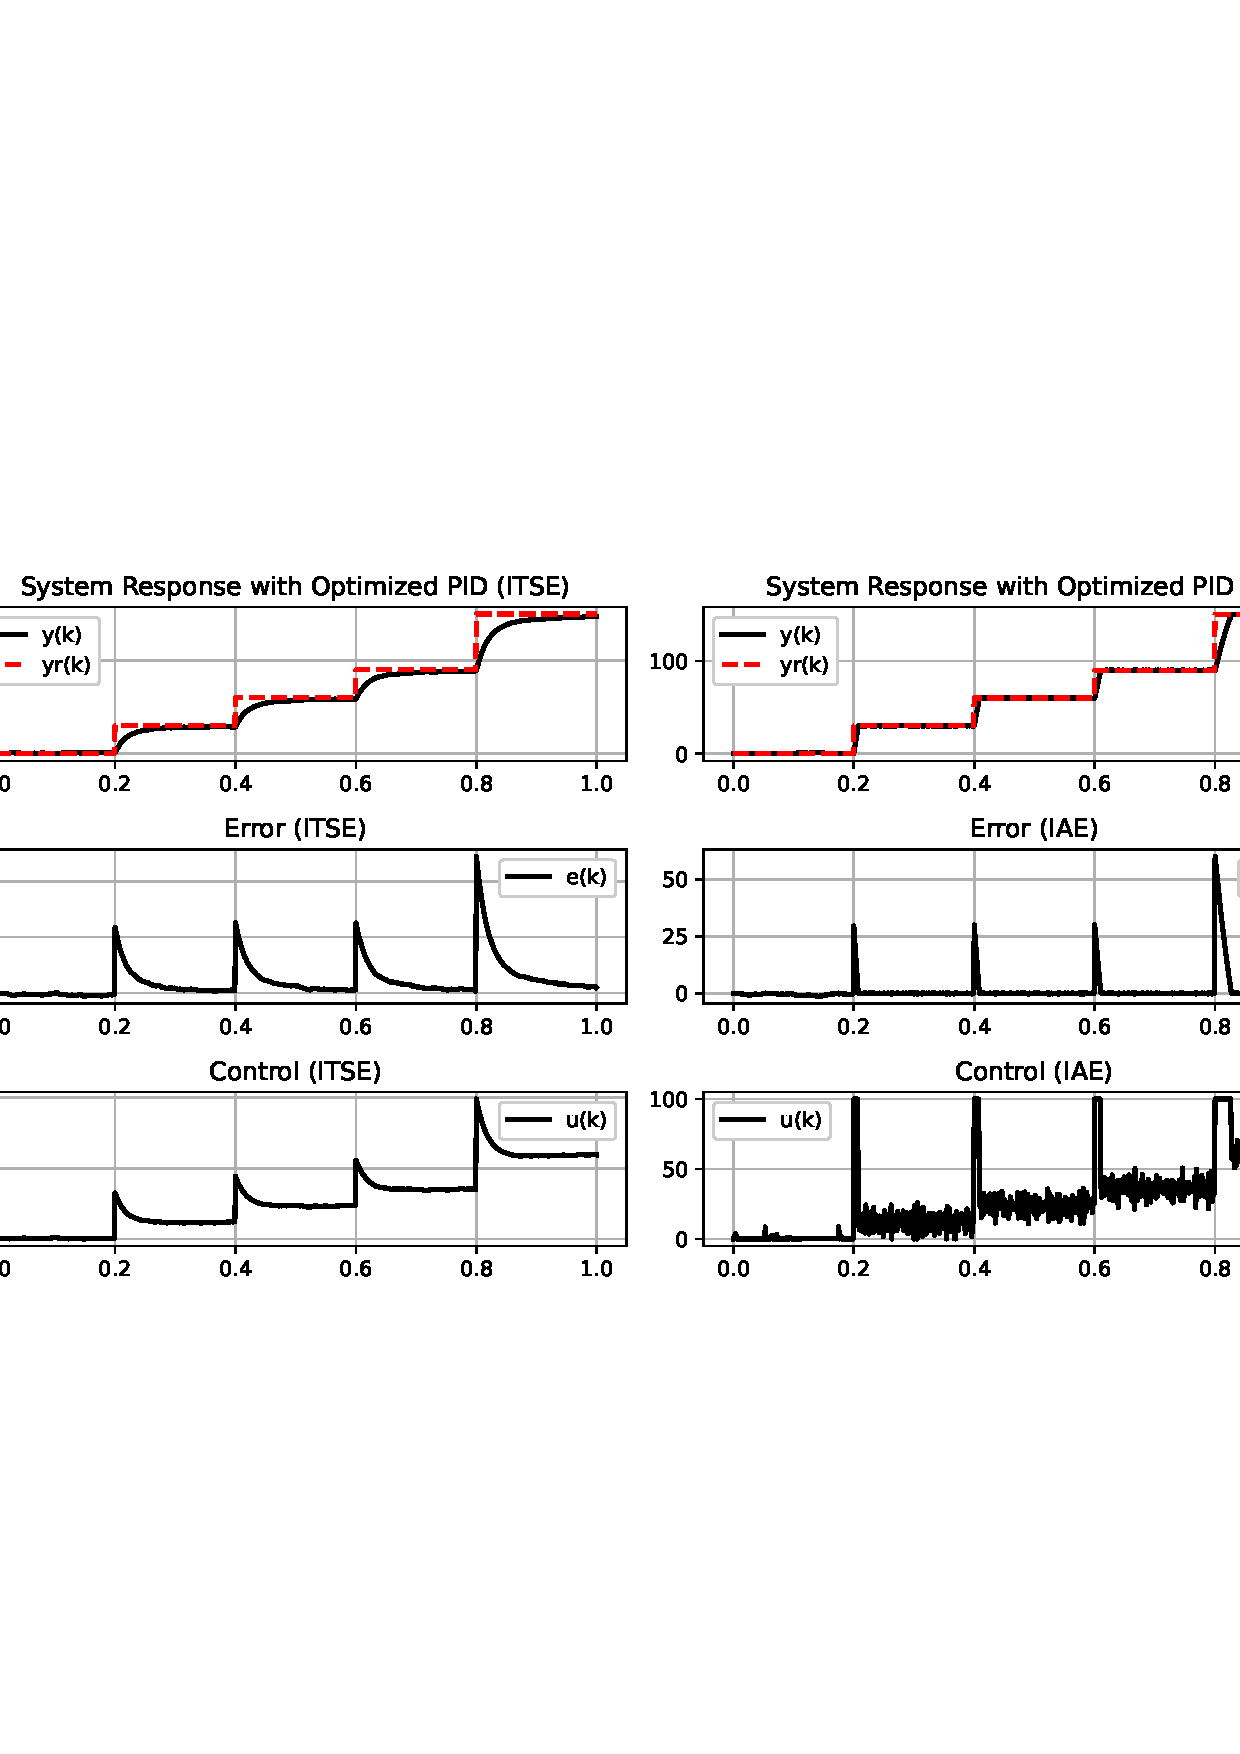
\includegraphics{images/Figure_6.png}}
    \caption{Respuesta del Sistema en Lazo Cerrado a Entrada Sinodal con una Frecuencia de 0.05 Hz}
    \label{fig:close_loop_sine_response}
\end{figure}

El análisis de los datos recopilados experimentalmente permiten observar que desfase de sistema desarrollado con respecto a una señal sinodal de 0.05 Hz es de 1.24° como se observa en la Figura~\ref{fig:close_loop_sine_response}.

\begin{figure}[H]
    \centering
    \resizebox{0.6\textwidth}{!}{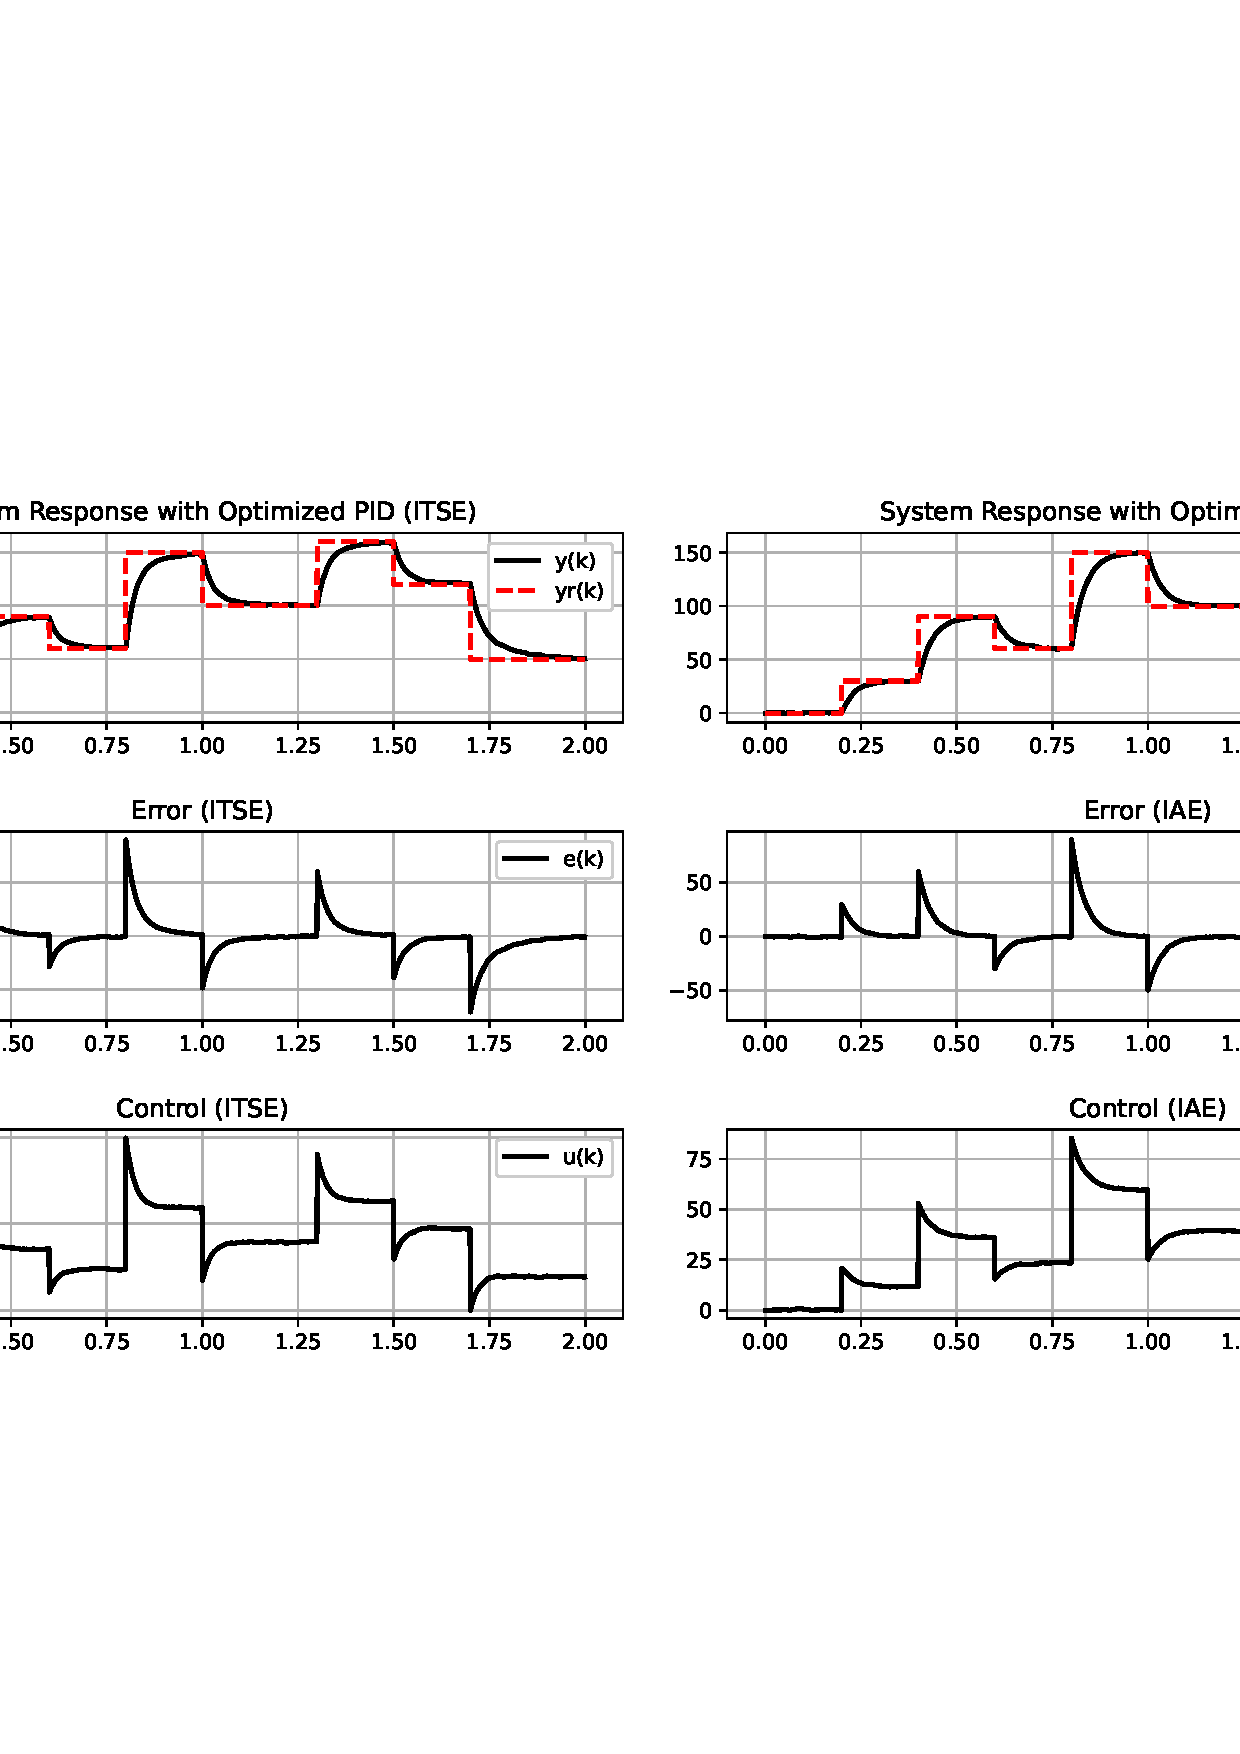
\includegraphics{images/Figure_7.png}}
    \caption{Respuesta del Sistema en Lazo Cerrado a Entrada Escalón}
    \label{fig:close_loop_step_response}
\end{figure}
Finalmente el analisis de la respuesta a escalón para un cambio de 20 RPM muestra un sobre impulso del 16.36\% tal y como se aprecia en la Figura~\ref{fig:close_loop_step_response}.

\section{Conclusión}
En este informe, se ha presentado la implementación de un controlador digital de bajo nivel para motores DC en el contexto de un laboratorio de ingeniería mecatrónica. A lo largo del trabajo, se han abordado varias etapas clave, desde la medición de la señal de entrada hasta la implementación y evaluación del controlador digital.

El proceso experimental comenzó con la medición de la señal de entrada, que era una señal sinusoidal generada por un programa simulador de generador de señales analógicas. Luego, se procedió a la supervisión del módulo de modulación por ancho de pulsos (PWM) para asegurar su correcto funcionamiento. Posteriormente, se implementó el control de pulsos del motor DC, calculando el ciclo de trabajo del PWM en función de la señal de entrada y la dirección de rotación del motor.

En la segunda parte del laboratorio, se desarrolló un sistema de lazo abierto para la planta, obteniendo su respuesta en frecuencia y sus dinámicas. Luego, se diseñó y sintonizó un controlador PID en configuración paralela mediante simulación, utilizando el modelo de la planta. Estos parámetros se transfirieron a la planta real después de corregir las discrepancias entre el modelo y la planta real.

Los resultados experimentales mostraron la respuesta del sistema en lazo cerrado a diferentes tipos de entrada, como señales sinusoidales y escalones. Se observó un desfase de sistema de 1.24° y un sobreimpulso del 16.36\% en la respuesta a escalón, lo que indica que el controlador digital logra un buen rendimiento en términos de seguimiento de referencia y estabilidad.

En resumen, este trabajo proporciona una visión detallada de la implementación de un controlador digital de bajo nivel para motores DC en un entorno de laboratorio de ingeniería mecatrónica. Se ha demostrado la importancia de la identificación del sistema, la sintonización del controlador y la corrección de las discrepancias entre el modelo y la planta real para lograr un rendimiento satisfactorio del sistema de control.

%\bibliographystyle{ieeetr}  
%\bibliography{library}

\end{document}
